\documentclass[a4paper,11pt]{article}
\usepackage[utf8x]{inputenc}      % input font encoding
\usepackage[lmargin=2.5cm,rmargin=2.5cm,tmargin=2.5cm,bmargin=3.5cm]{geometry}
\usepackage{amsmath,amssymb}
\usepackage[T1]{fontenc}          % output font encoding
\usepackage{booktabs,tabularx}
\usepackage{rotating}             % for sidewaystable
\usepackage{xspace}
\usepackage[usenames]{xcolor}
\usepackage{tikz,tikz-uml}
\usetikzlibrary{shapes,arrows,positioning}
\tikzstyle{block} = [rectangle, draw, text centered, minimum height=2em]
\tikzstyle{cloud} = [rectangle, draw, dashed, align=left, minimum height=2em]
\tikzstyle{arrow} = [draw, -latex, thick]
\tikzstyle{arrow2} = [draw, latex-latex, thick]
\tikzstyle{dashed-arrow} = [draw, -latex, dashed]
\usepackage{listings}             % source code highlighting
\lstset{breaklines=true,
  breakatwhitespace=true,
  stepnumber=1,
  basicstyle=\ttfamily\footnotesize,
  commentstyle=\ttfamily\color{gray},
  prebreak={\textbackslash},
  breakindent=10pt,
  breakautoindent=false,
  showspaces=false,
  showstringspaces=false,
  frame=single}
\usepackage[pdftitle={FlexibleSUSY --- A spectrum generator generator for supersymmetric models},
pdfauthor={Peter Athron,Jae-hyeon Park,Dominik Stockinger,Alexander Voigt},
pdfkeywords={FlexibleSUSY,supersymmetry,spectrum,generator,MSSM,NMSSM,E6SSM},
bookmarks=true, linktocpage]{hyperref}

\newcommand{\FlexibleSUSYVersion}{1.0.1\xspace}
\newcommand{\FlexibleSUSY}{FlexibleSUSY\xspace}


\newcommand{\sarah}{SARAH\xspace}
\newcommand{\flexisusy}{\FlexibleSUSY}

\newcommand{\code}[1]{\lstinline|#1|}  % inline source code
\newcommand{\unit}[1]{\;\text{#1}}       % units
\newcommand{\textoverline}[1]{$\overline{\mbox{#1}}$}
\newcommand{\DRbar}{\textoverline{DR}\xspace}
\newcommand{\MSbar}{\textoverline{MS}\xspace}
\newcommand{\userinput}{\text{<input>}}
\newcommand{\figref}[1]{\figurename~\ref{#1}}
\DeclareMathOperator{\re}{Re}
\DeclareMathOperator{\im}{Im}

\begin{document}

\begin{titlepage}
  \vspace*{55mm}
  \begin{center}
    {\Large\bf \FlexibleSUSY\ --- A spectrum generator generator for
      supersymmetric models}
    \\[8mm]
    Peter Athron$^{*}$,
    Jae-hyeon Park$^{\dagger}$,
    Dominik St\"ockinger$^{\dagger}$,
    Alexander Voigt$^{\dagger}$
    \\[3mm]
    {\small\it $^*$ ARC Centre of Excellence for Particle Physics at
      the Terascale, School of Chemistry and Physics, University of
      Adelaide, Adelaide, SA 5005, Australia,
      \\[2mm]
      \small\it $^\dagger$ Institut f\"ur Kern und Teilchenphysik, TU
      Dresden, Dresden, 01062, Germany.\\[2mm]}
  \end{center}
  \vspace*{0.75cm}
  \begin{abstract}
    We present FlexibleSUSY a new spectrum generator generator for
    supersymmetric models with modularity and speed in mind.
  \end{abstract}
  \vfill
  \begin{flushleft}
    \FlexibleSUSY version \FlexibleSUSYVersion
  \end{flushleft}
\end{titlepage}

\tableofcontents
\clearpage
\section{Overview}

FlexibleSUSY provides Mathematica and C++ code to create spectrum
generators for non-minimal supersymmetric models.

\subsection{Design goals}

FlexibleSUSY is designed with the following points in mind:

\paragraph{Speed}
Exploring the parameter space of supersymmetric models with a high
number of free parameters is quite time consuming.  Therefore
FlexibleSUSY aims to produce spectrum generators with a short run-time.

The two most time consuming parts of a spectrum generator are the
calculation of the beta functions and the pole masses for mixed
particles.

The reason is the following: The RG solving algorithms usually need
$O(10)$ iterations to calculate a particle spectrum with $0.1\%$
precision.  During each iteration the Runge--Kutta algorithm needs to
calculate all beta functions $O(50)$ times.  Most two-loop beta
functions involve $O(50)$ matrix multiplications and additions.  All
together one arrives at $O(2.5\cdot 10^4)$ matrix multiplications.  To
optimize these matrix multiplications FlexibleSUSY uses the fast
linear algebra package \href{Eigen}{http://eigen.tuxfamily.org}, which
exploits C++ expression templates to make the matrix multiplications
easy to write and optimize.

The second most time consuming part is the precise calculation of the
pole masses for mixed particles.  For each particle $\psi_i$ the full
self-energy matrix $\Sigma^\psi_{ij}(p=m^\text{tree}_{\psi_i})$ has to
be evaluated.  Each self-energy matrix entry again involves the
evaluation of $O(50)$ Feynman diagrams, which involves the calculation
of vertices and loop functions.  All in all, one arrives at $O(500)$
Feynman diagram or $O(3\cdot 10^4)$ loop function evaluations.  To
speed up the calculation of the pole masses FlexibleSUSY makes use of
multi-threading, where each pole mass is calculated in a separate
thread.  By this technique one can gain a speed-up of $20$--$30\%$.

\paragraph{Modularity}
The large variety of supersymmetric models makes it likely that the
user needs to modify the generated spectrum generator source code.
FlexibleSUSY uses object orientation with C++ to modularize the source
code to make it easy for the user to modify and extend the spectrum
generator.  An important application here are the constraints: The RG
solvers provide a constraint interface,
\figurename~\ref{fig:schematic-two-scale-constraint-interface},
%
\begin{figure}
  \centering
  \tikzumlset{fill class=white}
  \begin{tikzpicture}
    \umlclass[x=0, y=0]{RGFlow$<$Two\_scale$>$}{}{
      + solve()
    }
    \umlclass[x=6, y=0, type=abstract]{Constraint$<$Two\_scale$>$}{}{
      + \umlvirt{apply()}\\
      + \umlvirt{get\_scale() : double}
    }
    \umlclass[x=6, y=-3]{MyConstraint}{}{
      + apply()\\
      + get\_scale() : double
    }
    \umldep{RGFlow$<$Two\_scale$>$}{Constraint$<$Two\_scale$>$}
    \umlinherit{MyConstraint}{Constraint$<$Two\_scale$>$}
  \end{tikzpicture}
  \caption{Schematic two-scale constraint interface}
  \label{fig:schematic-two-scale-constraint-interface}
\end{figure}
%
which can be implemented to create the custom constraint
\code{MyConstraint}.  In the \code{apply()} function the constraint
application takes place and the \code{get_scale()} function specifies
the scale at which the constraint is to be applied.

\subsection{Requirements}

\begin{itemize}
\item Mathematica, version 7 or higher
\item SARAH, version 4.0.4 or higher \url{http://sarah.hepforge.org}
\item C++11 compatible compiler (g++ 4.4.7 or higher, clang++ 3.1 or
  higher)
\item Fortran compiler (gfortran, ifort etc.)
\item Eigen library, version 3.1 \url{http://eigen.tuxfamily.org}
\item Boost library, version 1.36.0 or higher
  \url{http://www.boost.org}
\item GNU scientific library \url{http://www.gnu.org/software/gsl/}
\item lapack (needed for the Lattice algorithm only)
  \url{http://www.netlib.org/lapack/}
\end{itemize}
%
Optional:
%
\begin{itemize}
\item Looptools, version 2.8 or higher
  \url{http://www.feynarts.de/looptools/}
\end{itemize}

\section{Quick start}
Create a MSSM spectrum generator
\begin{lstlisting}[language=bash]
./createmodel --name=NMSSM
./configure --with-models=NMSSM
make
\end{lstlisting}
Run the spectrum generator using the default parameter point
\begin{lstlisting}[language=bash]
./models/NMSSM/run_NMSSM.x
\end{lstlisting}
Run the spectrum generator using a SLHA input file
\begin{lstlisting}[language=bash]
./models/NMSSM/run_NMSSM.x \
   --slha-input-file=templates/NMSSM/LesHouches.in.NMSSM \
   --slha-output-file=LesHouches.out.NMSSM
\end{lstlisting}

\section{Usage}

\subsection{Workflow}

Creating a spectrum generator with \flexisusy consists of the
following steps:
%
\begin{enumerate}
  \setcounter{enumi}{-1}
\item Creating a \emph{SARAH model file}.  The SARAH model file must
  be loadable via \code{Start["<model-name>"]}.  Note, that SARAH
  already ships a lot of pre-defined model files in
  \code{SARAH/Models/} that can be used.
\item Creating a \emph{\flexisusy model file} in
  \code{models/<model-name>/}.  The \code{createmodel} script will
  help you creating one, see Section~\ref{sec:createmodel}.  For more
  details on how to write a \flexisusy model file see
  Section~\ref{sec:model-files}.
\item \emph{Configure} \flexisusy with your desired model, see
  Section~\ref{sec:configure}.
\item Run \code{make}.  This will create the C++ code for your
  spectrum generator and compile it, see Section~\ref{sec:make}.
\end{enumerate}
%
The steps 1--3 are illustrated in \figref{fig:workflow}.

\begin{figure}[tbh]
  \centering
  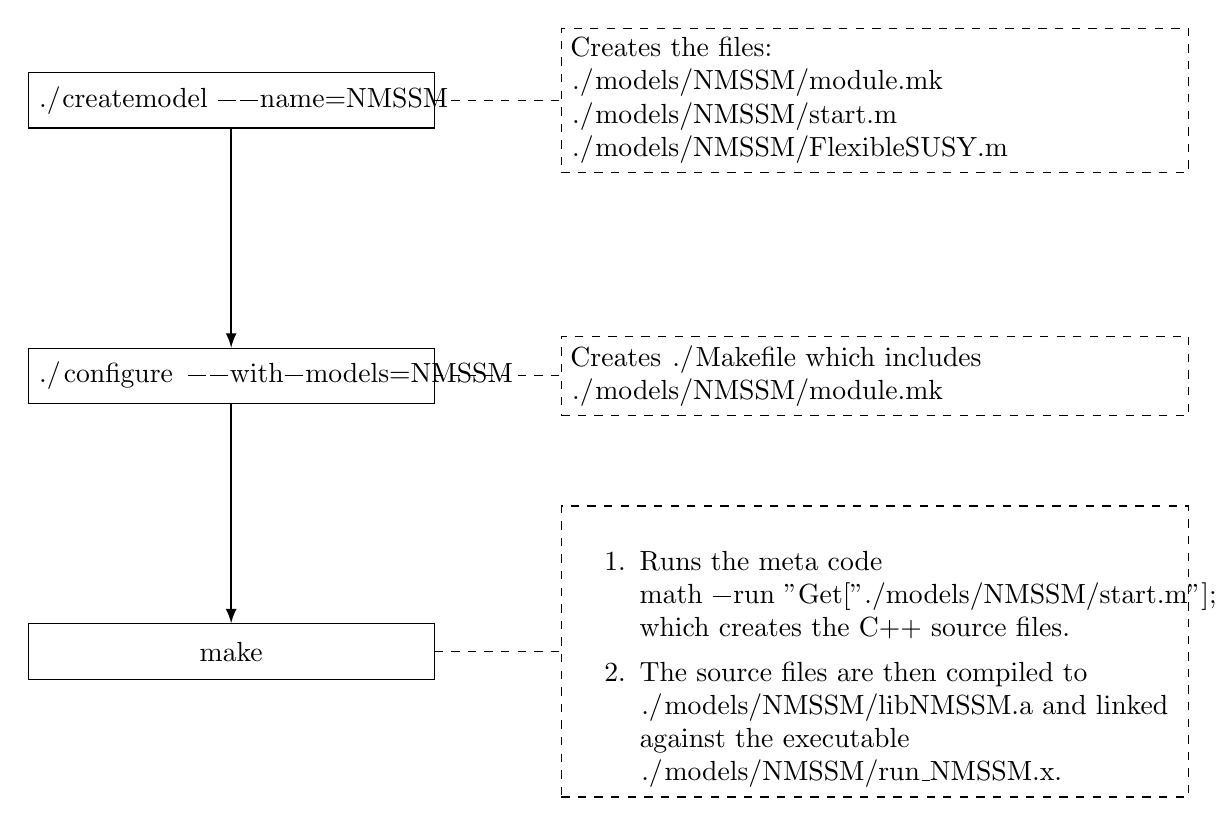
\begin{tikzpicture}[node distance = 3.5cm, auto]
    \node[block, text width=14em] (createmodel) {%
      \code{./createmodel --name=NMSSM}};
    \node[block, text width=14em, below of=createmodel] (configure) {%
      \code{./configure --with-models=NMSSM}};
    \node[block, text width=14em, below of=configure] (make) {%
      \code{make}};
    \node[cloud, text width=22em, right=1.6cm of createmodel] (createmodel-output) {%
      Creates the files:\\%
      \code{./models/NMSSM/module.mk}\\%
      \code{./models/NMSSM/start.m}\\%
      \code{./models/NMSSM/FlexibleSUSY.m}};
    \node[cloud, text width=22em, right=1.6cm of configure] (configure-output) {%
      Creates \code{./Makefile} which includes\\%
      \code{./models/NMSSM/module.mk}};
    \node[cloud, text width=22em, right=1.6cm of make] (make-output) {%
      \begin{enumerate}\itemsep0em
      \item Runs the meta code \code{math -run
          "Get[\"./models/NMSSM/start.m\"];"} which creates the C++
        source files.
      \item The source files are then compiled to
        \code{./models/NMSSM/libNMSSM.a} and linked against the
        executable \code{./models/NMSSM/run\_NMSSM.x}.
      \end{enumerate}};
    \path[arrow] (createmodel) -- (configure);
    \path[arrow] (configure) -- (make);
    \path[draw, dashed] (createmodel) -- (createmodel-output);
    \path[draw, dashed] (configure) -- (configure-output);
    \path[draw, dashed] (make) -- (make-output);
  \end{tikzpicture}
  \caption{\flexisusy workflow}
  \label{fig:workflow}
\end{figure}

\subsection{Basic commands}

Explain:
\begin{itemize}
\item ./createmodel
\item ./configure
\item make
\item Mathematica interface (see models/<model>/start.m)
\end{itemize}

\subsubsection{\code{createmodel}}
\label{sec:createmodel}

The \code{createmodel} script sets up a \flexisusy\ model.  This involves
%
\begin{itemize}
\item a model directory \code{models/<flexiblesusy-model>/}
\item a makefile module \code{models/<flexiblesusy-model>/module.mk}
\item a \flexisusy\ model file \code{models/<flexiblesusy-model>/FlexibleSUSY.m}
\item a Mathematica start script \code{models/<flexiblesusy-model>/start.m}
\end{itemize}
%
Usage:
\begin{lstlisting}[language=bash]
./createmodel --name=<flexiblesusy-model> --sarah-model=<sarah-model>
\end{lstlisting}
Here \code{<flexiblesusy-model>} is the name of \flexisusy\ model
to be created and \code{<sarah-model>} is the name of the \sarah\
model file which defines the Lagrangian and the particles.\\
Example:
\begin{lstlisting}[language=bash]
./createmodel --name=MyCMSSM --sarah-model=MSSM
\end{lstlisting}
%
%
If a certain \sarah\ sub-model should be used, the name of the sub-model
has to be appended with at preceeding slash.\\
Example: use the \code{CKM} sub-model of the \code{MSSM}
\begin{lstlisting}[language=bash]
./createmodel --name=MyCMSSM --sarah-model=MSSM/CKM
\end{lstlisting}
%
For further information and options see
\begin{lstlisting}[language=bash]
./createmodel --help
\end{lstlisting}

\subsubsection{\code{configure}}
\label{sec:configure}

The \code{configure} script checks for the installed compilers,
libraries and Mathematica.  If all of these exists in a sufficent
version, the \code{Makefile} is created, which contains the information
on how to compile the code.  The user has to specify the models which
should be included in the build via the \code{--with-models=} option,
e.g.
%
\begin{lstlisting}[language=bash]
./configure --with-models=<flexibsusy-model>
\end{lstlisting}
%
Here \code{<flexibsusy-model>} is either \code{all} or a comma
separated list of \flexisusy models.

Furthermore, the user can select which RG solver algorithms to use via
the \code{--with-algorithms=} option.\\
Example:
%
\begin{lstlisting}[language=bash]
./configure --with-algorithms=two_scale
\end{lstlisting}

The \code{configure} script further allows to select the C++ and
Fortran compilers, the Mathematica kernel command as well as paths to
libraries and header files.  See
\code{configure --help} for all available options.\\
Example:
%
\begin{lstlisting}[language=bash]
./configure --with-models=MSSM --with-cxx=clang++
   --with-boost-incdir=/usr/include/
   --with-boost-libdir=/usr/lib/
\end{lstlisting}

\subsubsection{\code{make}}
\label{sec:make}

Running \code{make} will create the C++ source code for your spectrum
generator and compile it.  These two processes are controled in the
makefile module \code{models/<model-name>/module.mk}.  See,
Section~\ref{sec:makefile-modules} for details how to create your own
makefile module.

\subsection{Model files}
\label{sec:model-files}

Explain how to write a \flexisusy\ model file (starting from a \sarah\
model file).

A \flexisusy\ model file is a Mathematica file, where the following
pieces are defined:

\paragraph{General model information}

\subparagraph{FSModelName}
Name of the \flexisusy\ model.
Example (MSSM):
\begin{lstlisting}[language=Mathematica]
FSModelName = "MSSM";
\end{lstlisting}

\subparagraph{OnlyLowEnergyFlexibleSUSY} If set to True, creates a
spectrum generator without high-scale constraint, i.e.\ only a
low-scale and susy-scale constraint will be created (default: False).
In this case all model parameters, except for gauge and Yukawa
couplings are input at the susy scale.  This option is similar to
\code{OnlyLowEnergySPheno} in SARAH/SPheno.
\\
Example:
\begin{lstlisting}[language=Mathematica]
OnlyLowEnergyFlexibleSUSY = False;  (* default *)
\end{lstlisting}

\paragraph{Input and output parameters}

\subparagraph{MINPAR} This list of two-component lists defines model
input parameters and their SLHA keys.  These parameters will be read
from the MINPAR block in the SLHA file.
\\
Example (MSSM):
\begin{lstlisting}[language=Mathematica]
MINPAR = { {1, m0},
           {2, m12},
           {3, TanBeta},
           {4, Sign[\[Mu]]},
           {5, Azero}
         };
\end{lstlisting}

\subparagraph{EXPAR} This list of two-component lists defines further
model input parameters and their SLHA keys.  These parameters will be
read from the EXTPAR block in the SLHA file.
\\
Example (E6SSM):
\begin{lstlisting}[language=Mathematica]
EXTPAR = { {61, LambdaInput},
           {62, KappaInput},
           {63, muPrimeInput},
           {64, BmuPrimeInput},
           {65, vSInput}
         };
\end{lstlisting}

\paragraph{Constraints}
Currently three constraints are supported: low-scale, susy-scale and
high-scale constraints.  In \flexisusy\ they are named as
\code{LowScale}, \code{SUSYScale} and \code{HighScale}.  For
each constraint there is a scale definition (named after the
constraint), an initial guess for the scale (concatenation of the
constraint name and \code{FirstGuess}) and a list settings to be
applied at the constraint (concatenation of the constraint name and
\code{Input}).
\\
Example (MSSM):
\begin{lstlisting}[language=Mathematica]
(* susy-scale constraint *)
SUSYScale = Sqrt[M[Su[1]]*M[Su[6]]];        (* scale definition *)
SUSYScaleFirstGuess = Sqrt[m0^2 + 4 m12^2]; (* first scale guess *)
SUSYScaleInput = {};                        (* nothing is set here *)

(* high-scale constraint *)
HighScale = g1 == g2;                       (* scale definition *)
HighScaleFirstGuess = 2.0 10^16;            (* first scale guess *)
HighScaleInput = {
   {T[Ye], Azero*Ye},
   {T[Yd], Azero*Yd},
   {T[Yu], Azero*Yu},
   {mHd2, m0^2},
   {mHu2, m0^2},
   {mq2, UNITMATRIX[3] m0^2},
   {ml2, UNITMATRIX[3] m0^2},
   {md2, UNITMATRIX[3] m0^2},
   {mu2, UNITMATRIX[3] m0^2},
   {me2, UNITMATRIX[3] m0^2},
   {MassB, m12},
   {MassWB,m12},
   {MassG, m12}
};

LowScale = LowEnergyConstant[MZ];           (* scale definition *)
LowScaleFirstGuess = LowEnergyConstant[MZ]; (* first scale guess *)
LowScaleInput = {
   {vd, 2 MZDRbar / Sqrt[GUTNormalization[g1]^2 g1^2 + g2^2] Cos[ArcTan[TanBeta]]},
   {vu, 2 MZDRbar / Sqrt[GUTNormalization[g1]^2 g1^2 + g2^2] Sin[ArcTan[TanBeta]]}
};
\end{lstlisting}

\paragraph{Initial parameter guesses} At the \code{LowScale} and
\code{HighScale} it is recommended to make an initial guess for the
model parameters.  This can be done via
\begin{lstlisting}[language=Mathematica]
InitialGuessAtLowScale = {
   {vd, LowEnergyConstant[vev] Cos[ArcTan[TanBeta]]},
   {vu, LowEnergyConstant[vev] Sin[ArcTan[TanBeta]]}
};

InitialGuessAtHighScale = {
   {\[Mu]   , 1.0},
   {B[\[Mu]], 0.0}
};
\end{lstlisting}

\paragraph{Setting the tree-level EWSB eqs.\ solution by hand} In case
the meta code cannot find an analytic solution to the tree-level EWSB
eqs., one can set solutions by hand in the model file using the
variable \code{TreeLevelEWSBSolution}.
\\
Example (MSSM):
\begin{lstlisting}[language=Mathematica]
TreeLevelEWSBSolution = {
  {\[Mu]   , ... },
  {B[\[Mu]], ... }
};
\end{lstlisting}

\begin{sidewaystable}[tb]
  \centering
  \begin{tabularx}{\textwidth}{>{\ttfamily}l>{\ttfamily}lX}
    \toprule
    variable    & default value & description \\
    \midrule
    FSModelName & Model`Name & Name of the \flexisusy\ model \\
    OnlyLowEnergyFlexibleSUSY & False & low-energy model \\
    MINPAR & \{\} & list of input parameters in SLHA MINPAR block \\
    EXTPAR & \{\} & list of input parameters in SLHA EXTPAR block \\
    LowScale & LowEnergyConstant[MZ] & Standard Model matching scale (in GeV) \\
    LowScaleFirstGuess & LowEnergyConstant[MZ] & first guess for the Standard Model matching scale (in GeV) \\
    LowScaleInput & \{\} & settings applied at the low scale \\
    SUSYScale & 1000 & scale of supersymmetric particle masses (in GeV) \\
    SUSYScaleFirstGuess & 1000 & first guess for the susy scale (in GeV) \\
    SUSYScaleInput & \{\} & settings applied at the susy scale \\
    HighScale & SARAH`hyperchargeCoupling == SARAH`leftCoupling
      & unification scale (in GeV) \\
    HighScaleFirstGuess & $2\cdot 10^{16}$ & first guess for the unification scale (in GeV) \\
    HighScaleInput & \{\} & settings applied at the unification scale \\
    \bottomrule
  \end{tabularx}
  \caption{\flexisusy\ model file variables}
  \label{tab:model-file-variables}
\end{sidewaystable}

\subsection{Makefile modules}
\label{sec:makefile-modules}

Explain how to write a custom makefile module (module.mk) for a
\flexisusy\ model.

\section{Output}
\subsection{Files}

Explain the created C++ files and executables, and how to use them.

\subsection{Two-scale algorithm}

Explain the structure of the two-scale algorithm classes and how they
work and are plugged together.


The stucture of the two-scale algorithm used in \flexisusy\ is as follows,%

Initial guess:
\begin{enumerate}
\item Guess gauge couplings $g_{1,2,3}$ at $m_Z$
\item Apply user-defined low-scale constraint (\code{LowScaleInput})
\item Guess Yukawa couplings $y^{u,d,e}_{ij}$ at $m_Z$
\item Run model to the high-scale (\code{HighScaleFirstGuess})
\item Apply high-scale constraint (\code{HighScaleInput})
\item Run model to the low-scale (\code{LowScaleFirstGuess})
\item Solve EWSB eqs.\ at the tree-level
\item Calculate \DRbar\ masses
\end{enumerate}
%
Solving the renormalization group equations:
\begin{enumerate}
\item \label{rge-step-one} Run model to the low-scale (\code{LowScale})
  \begin{enumerate}
  \item Calculate \DRbar\ masses
  \item Recalculate low-scale
  \item Calculate \DRbar\ gauge and Yukawa couplings $g_{1,2,3}$,
    $y^{u,d,e}_{ij}$, see
    Section~\ref{sec:matching-to-the-standard-model}.
  \item Apply user-defined low-scale constraint (\code{LowScaleInput})
  \end{enumerate}
\item Run model to the high-scale (\code{HighScale})
  \begin{enumerate}
  \item Recalculate high-scale
  \item Apply high-scale constraint (\code{HighScaleInput})
  \end{enumerate}
\item Run model to the susy-scale (\code{SUSYScale})
  \begin{enumerate}
  \item Calculate \DRbar\ masses
  \item Recalculate low-scale
  \item Apply susy-scale constraint (\code{SUSYScaleInput})
  \item Solve EWSB eqs.\ at the one-loop level
  \end{enumerate}
\item If not converged yet, goto \ref{rge-step-one}
\end{enumerate}
%
Calculating the particle spectrum:
\begin{enumerate}
\item Run model to the susy-scale
\item Calculate the pole masses
\item Run model to the parameter output scale (SLHA block MODSEL 12)
\end{enumerate}

\begin{figure}[tb]
  \centering
  \tikzumlset{fill class=white}
  \begin{tikzpicture}
    \umlclass[x=0, y=0, type=abstract]{Beta\_function}{
      -- scale : double\\
      -- loops : unsigned\\
      -- numPars : unsigned
    }{
      + \umlvirt{display() : const Eigen::ArrayXd} \\
      + \umlvirt{set(v : const Eigen::ArrayXd\&) : void}\\
      + \umlvirt{beta() : Eigen::ArrayXd}\\
      + run\_to(scale : double, eps : double) : void\\
    }
    \umlclass[x=8, y=-12, template={T}]{MSSM}{}{}
    \umlclass[x=8, y=-8, type=abstract]{Two\_scale\_model}{}{
      + \umlvirt{calculate\_spectrum() : void}\\
      + \umlvirt{run\_to(scale : double, eps : double) : void}\\
      + \umlvirt{set\_precision(precision : double) : void}
    }
    \umlclass[x=0, y=-4]{MSSM\_susy\_parameters}{}{
      + display() : const Eigen::ArrayXd \\
      + set(v : const Eigen::ArrayXd\&) : void\\
      + beta() : Eigen::ArrayXd
    }
    \umlclass[x=0, y=-8]{MSSM\_soft\_parameters}{}{
      + display() : const Eigen::ArrayXd \\
      + set(v : const Eigen::ArrayXd\&) : void\\
      + beta() : Eigen::ArrayXd
    }
    \umlclass[x=0, y=-12]{MSSM$<$Two\_scale$>$}{}{
      + calculate\_spectrum() : void\\
      + run\_to(scale : double, eps : double) : void\\
      + set\_precision(precision : double) : void
    }
   \umlinherit{MSSM\_susy\_parameters}{Beta\_function}
   \umlinherit{MSSM\_soft\_parameters}{MSSM\_susy\_parameters}
   \umlinherit{MSSM$<$Two\_scale$>$}{MSSM\_soft\_parameters}
   \umlinherit{MSSM$<$Two\_scale$>$}{Two\_scale\_model}
   \umldep[arg1={$<<$bind$>>$}, mult1={T $\rightarrow$ Two\_scale}, pos1=0.5]{MSSM$<$Two\_scale$>$}{MSSM}
  \end{tikzpicture}
  \caption{Two-scale model class hierarchy}
  \label{fig:two-scale-model-class-hierarchy}
\end{figure}

\begin{figure}[tb]
  \centering
  \tikzumlset{fill class=white}
  \begin{tikzpicture}
    \umlclass[x=0, y=0, type=abstract]{Two\_scale\_model}{}{
      + \umlvirt{calculate\_spectrum() : void}\\
      + \umlvirt{run\_to(scale : double, eps : double) : void}\\
      + \umlvirt{set\_precision(precision : double) : void}
    }
    \umlclass[x=0, y=-4]{RGFlow$<$Two\_scale$>$}{}{
      + solve() : void
    }
    \umlclass[x=8, y=0]{Constraint$<$Two\_scale$>$}{}{
      + \umlvirt{apply() : void}\\
      + \umlvirt{get\_scale() : double}\\
      + \umlvirt{set\_model(model : Two\_scale\_model*) : void}
    }
    \umlclass[x=8, y=4, template={T}]{Constraint}{}{}
    \umlclass[x=0, y=-7]{Initial\_guesser$<$Two\_scale$>$}{}{
      + \umlvirt{guess() : void}
    }
    \umlclass[x=0, y=-11, template={T}]{Initial\_guesser}{}{}
    \umlclass[x=8, y=-7]{Convergence\_tester$<$Two\_scale$>$}{}{
      + \umlvirt{accuracy\_goal\_reached() : bool}\\
      + \umlvirt{max\_iterations() : unsigned}
    }
    \umlclass[x=8, y=-11, template={T}]{Convergence\_tester}{}{}
    \umlclass[x=8, y=-4, template={T}]{RGFlow}{}{}
    \umldep[arg1={$<<$bind$>>$}, mult1={T $\rightarrow$ Two\_scale}, pos1=0.5]{RGFlow$<$Two\_scale$>$}{RGFlow}
    \umldep[mult1=1..*]{RGFlow$<$Two\_scale$>$}{Two\_scale\_model}
    \umldep[mult1=1..*]{RGFlow$<$Two\_scale$>$}{Constraint$<$Two\_scale$>$}
    \umldep{RGFlow$<$Two\_scale$>$}{Initial\_guesser$<$Two\_scale$>$}
    \umldep{RGFlow$<$Two\_scale$>$}{Convergence\_tester$<$Two\_scale$>$}
    \umldep[mult1={$<<$bind$>>$}, arg1={T $\rightarrow$ Two\_scale}, pos1=0.5]{Initial\_guesser$<$Two\_scale$>$}{Initial\_guesser}
    \umldep[mult1={$<<$bind$>>$}, arg1={T $\rightarrow$ Two\_scale}, pos1=0.5]{Convergence\_tester$<$Two\_scale$>$}{Convergence\_tester}
    \umldep[arg1={$<<$bind$>>$}, mult1={T $\rightarrow$ Two\_scale}, pos1=0.5]{Constraint$<$Two\_scale$>$}{Constraint}
  \end{tikzpicture}
  \caption{Two-scale renormalization group solver class hierarchy}
  \label{fig:two-scale-rgflow-class-hierarchy}
\end{figure}

\subsubsection{Matching to the Standard Model}
\label{sec:matching-to-the-standard-model}

\paragraph{Gauge couplings}

At the low-scale $M_Z$ we calculate
%
\begin{align}
  \alpha_{\text{e.m.},\text{susy}}^{\text{\DRbar}}(M_Z) &=
  \frac{\alpha_{\text{e.m.},\text{SM}}^{(5),\text{\MSbar}}(M_Z)}{1 -
    \Delta\alpha_{\text{e.m.},\text{SM}}(M_Z) -
    \Delta\alpha_{\text{e.m.},\text{susy}}(M_Z)} ,\\
  \Delta\alpha_{\text{e.m.},\text{SM}}(\mu) &=
  \frac{\alpha_\text{e.m.}}{2\pi} \left[\frac{1}{3}
    - \frac{16}{9} \log{\frac{m_t}{\mu}} \right],\\
  \Delta\alpha_{\text{e.m.},\text{susy}}(\mu) &=
  \frac{\alpha_\text{e.m.}}{2\pi} \left[ -\sum_{\text{susy particle }
      i}
    C_i \log{\frac{m_i}{\mu}} \right],\\
    e_{\text{susy}}^{\text{\DRbar}}(M_Z) &=
    \sqrt{4\pi\alpha_{\text{e.m.},\text{susy}}^{\text{\DRbar}}(M_Z)}
\end{align}
%
\begin{align}
  \alpha_{\text{s},\text{susy}}^{\text{\DRbar}}(M_Z) &=
  \frac{\alpha_{\text{s},\text{SM}}^{(5),\text{\MSbar}}(M_Z)}{1 -
    \Delta\alpha_{\text{s},\text{SM}}(M_Z)
    - \Delta\alpha_{\text{s},\text{susy}}(M_Z)} ,\\
  \Delta\alpha_{\text{s},\text{SM}}(\mu) &=
  \frac{\alpha_\text{s}}{2\pi} \left[
    -\frac{2}{3} \log{\frac{m_t}{\mu}} \right],\\
  \Delta\alpha_{\text{s},\text{susy}}(\mu) &=
  \frac{\alpha_\text{s}}{2\pi}\left[ \frac{1}{2}-\sum_{\text{susy
        particle } i} C_i \log{\frac{m_i}{\mu}} \right] ,\\
  g_{3,\text{susy}}^{\text{\DRbar}}(M_Z) &=
  \sqrt{4\pi\alpha_{\text{s},\text{susy}}^{\text{\DRbar}}(M_Z)} ,
\end{align}
%
where
%
\begin{align}
  \alpha_{\text{e.m.},\text{SM}}^{(5),\text{\MSbar}}(M_Z) &= 1/127.944,\\
  \alpha_{\text{s},\text{SM}}^{(5),\text{\MSbar}}(M_Z) &= 0.1185,
\end{align}
%
are the \MSbar electromagnetic and strong cougling constants in the
Standard Model including only $5$ quark flavours
\cite{Beringer:1900zz}.  Afterwards, SARAH's tree-level expressions
for the Weinberg angle and the Hypercharge and left gauge couplings
$g_Y$ and $g_2$ in terms of $M_{W,\text{susy}}^{\text{\DRbar}}(M_Z)$,
$M_{Z,\text{susy}}^{\text{\DRbar}}(M_Z)$ and
$e_{\text{susy}}^{\text{\DRbar}}(M_Z)$ are used to calculate
$g_{1,\text{susy}}^{\text{\DRbar}}(M_Z)$ and
$g_{2,\text{susy}}^{\text{\DRbar}}(M_Z)$.  In the MSSM, for example,
we'll have
%
\begin{align}
  \theta_{W,\text{susy}}^{\text{\DRbar}}(M_Z) &=
  \arcsin\sqrt{1 - \left(\frac{M_{W,\text{susy}}^{\text{\DRbar}}(M_Z)}{M_{Z,\text{susy}}^{\text{\DRbar}}(M_Z)}\right)^2} ,\\
  g_{1,\text{susy}}^{\text{\DRbar}}(M_Z) &=
  \sqrt{\frac{5}{3}} \frac{e_{\text{susy}}^{\text{\DRbar}}(M_Z)}{\cos\theta_{W,\text{susy}}^{\text{\DRbar}}(M_Z)} ,\\
  g_{2,\text{susy}}^{\text{\DRbar}}(M_Z) &=
  \frac{e_{\text{susy}}^{\text{\DRbar}}(M_Z)}{\sin\theta_{W,\text{susy}}^{\text{\DRbar}}(M_Z)} ,
\end{align}
%
where
%
\begin{align}
  \left(M_{W,\text{susy}}^{\text{\DRbar}}(M_Z)\right)^2 &=
  \left(M_W^{\text{pole}}\right)^2 + \re \Pi_{WW}^T(p^2 = (M_W^{\text{pole}})^2) ,\\
  \left(M_{Z,\text{susy}}^{\text{\DRbar}}(M_Z)\right)^2 &=
  \left(M_Z^{\text{pole}}\right)^2 + \re \Pi_{ZZ}^T(p^2 = (M_Z^{\text{pole}})^2)
\end{align}
%
and $M_W^{\text{pole}} = 80.404\unit{GeV}$, $M_Z^{\text{pole}} =
91.1876\unit{GeV}$ \cite{Beringer:1900zz}.

\paragraph{Fermion masses}

The expressions for the SM-Yukawa coupling matrices extracted from the
tree-level mass matrices of the SM-fermions.  In the MSSM, for
example, they read
%
\begin{align}
  y_u^{\text{\DRbar}}(M_Z) &= \frac{\sqrt{2} m_{u}^T}{v_u} , &
  y_d^{\text{\DRbar}}(M_Z) &= \frac{\sqrt{2} m_{d}^T}{v_d} , &
  y_e^{\text{\DRbar}}(M_Z) &= \frac{\sqrt{2} m_{e}^T}{v_d}.
\end{align}
%
At the low-scale the fermion mass matrices are composed as
%
\begin{align}
  m_u =
  \begin{pmatrix}
    m_{u}^{\userinput} & 0 & 0 \\
    0 & m_{c}^{\userinput} & 0 \\
    0 & 0 & m_{t,\text{susy}}^{\text{\DRbar}}(M_Z)
  \end{pmatrix} ,\\
  m_d =
  \begin{pmatrix}
    m_{d}^{\userinput} & 0 & 0 \\
    0 & m_{s}^{\userinput} & 0 \\
    0 & 0 & m_{b,\text{susy}}^{\text{\DRbar}}(M_Z)
  \end{pmatrix} ,\\
  m_e =
  \begin{pmatrix}
    m_{e}^{\userinput} & 0 & \\
    0 & m_{\mu}^{\userinput} & 0 \\
    0 & 0 & m_{\tau,\text{susy}}^{\text{\DRbar}}(M_Z)
  \end{pmatrix}.
\end{align}
%
Only the 3rd generation quark masses are calculated in the \DRbar
scheme from the user input quantities $m_t^\text{pole}$,
$m_{b,\text{SM}}^{\text{\MSbar}}(M_Z)$,
$m_{\tau,\text{SM}}^{\text{\MSbar}}(M_Z)$.  In detail, the top quark
\DRbar mass is calculated via
%
\begin{align}
  \begin{split}
    m_{t,\text{susy}}^{\text{\DRbar}}(\mu) &= m_t^\text{pole} +
    \re\Sigma_{tt}^{S,\text{heavy}}(m_t^\text{pole}) \\
    &\phantom{=\;} + m_t^\text{pole}
    \left[ \re\Sigma_{tt}^{L,\text{heavy}}(m_t^\text{pole}) +
      \re\Sigma_{tt}^{R,\text{heavy}}(m_t^\text{pole}) + \Delta
      m_t^{(1),\text{qcd}} + \Delta m_t^{(2),\text{qcd}} \right] ,
  \end{split}
\end{align}
%
where the $\Sigma_{ff}^\text{heavy}$ denotes the self-energy of
fermion $f$ without the Standard Model contributions.  The appearing
QCD corrections $\Delta m_t^{(1),\text{qcd}}$ and $\Delta
m_t^{(2),\text{qcd}}$ are taken from
\cite[Eq. (58),(61)]{Bednyakov:2002sf} and read
%
\begin{align}
  \Delta m_t^{(1),\text{qcd}} &= -\frac{g_3^2 \left(5-3 \log\left(\frac{m_t^2}{\mu^2}\right)\right)}{12 \pi^2},\\
  \begin{split}
    \Delta m_t^{(2),\text{qcd}} &= \left(\Delta
      m_t^{(1),\text{qcd}}\right)^2 \\
    &\phantom{=\;} - \frac{g_3^4 \left[396
        \log^2\left(\frac{m_t^2}{\mu^2}\right)-1476
        \log\left(\frac{m_t^2}{\mu^2}\right)-48 \zeta(3)+2011+16 \pi
        ^2 (1+\log 4)\right]}{4608 \pi^4}.
  \end{split}
\end{align}
%
The \DRbar mass of the bottom quark is calculated via
\cite{Baer:2002ek,Skands:2003cj}
%
\begin{align}
  m_{b,\text{susy}}^{\text{\DRbar}}(\mu) &=
  \frac{m_{b,\text{SM}}^{\text{\DRbar}}(\mu)}{1 -
    \re\Sigma_{bb}^{S,\text{heavy}}(m_{b,\text{SM}}^\text{\MSbar})/m_b
    - \re\Sigma_{bb}^{L,\text{heavy}}(m_{b,\text{SM}}^\text{\MSbar}) -
    \re\Sigma_{bb}^{R,\text{heavy}}(m_{b,\text{SM}}^\text{\MSbar})} ,\\
  m_{b,\text{SM}}^{\text{\DRbar}}(\mu) &=
  m_{b,\text{SM}}^{\text{\MSbar}}(\mu) \left(1 - \frac{\alpha_s}{3
      \pi} - \frac{23}{72} \frac{\alpha_s^2}{\pi^2} + \frac{3
      g_2^2}{128 \pi^2} + \frac{13 g_Y^2}{1152 \pi^2}\right) ,
\end{align}
%
where $m_{b,\text{SM}}^{\text{\MSbar}}(M_Z)$ is user input.  The
\DRbar mass of the $\tau$ is calculated via
%
\begin{align}
  \begin{split}
    m_{\tau,\text{susy}}^{\text{\DRbar}}(\mu) &=
    m_{\tau,\text{SM}}^{\text{\DRbar}}(\mu) +
    \re\Sigma_{\tau\tau}^{S,\text{heavy}}(m_{\tau,\text{SM}}^\text{\MSbar}) \\
    &\phantom{=\;} + m_{\tau,\text{SM}}^{\text{\DRbar}}(\mu) \left[
      \re\Sigma_{\tau\tau}^{L,\text{heavy}}(m_{\tau,\text{SM}}^\text{\MSbar})
      +
      \re\Sigma_{\tau\tau}^{R,\text{heavy}}(m_{\tau,\text{SM}}^\text{\MSbar})
    \right] ,
  \end{split}\\
  m_{\tau,\text{SM}}^{\text{\DRbar}}(\mu) &= m_{\tau,\text{SM}}^{\text{\MSbar}}(\mu)
  \left(1 - 3 \frac{g_Y^2 - g_2^2}{128 \pi^2}\right),
\end{align}
%
where $m_{\tau,\text{SM}}^{\text{\MSbar}}(M_Z)$ is user input.  To
convert the fermion masses from the \MSbar to the \DRbar scheme the
Yukawa coupling conversion from \cite[Eq.~(19)]{Skands:2003cj} was
used and it was assumed that the VEV is already given in the \DRbar
scheme.

\subsection{Lattice algorithm}

Explain the structure of the lattice algorithm classes and how they
work.


%%%%%%%%%%%%%%%%%%%%%%%%%%%%%%%%%%%%%%%%%%%%%%%%%%%%%%%%%%%%%%%%%%%%%%%%%%%%%
% Bibliography

\clearpage
\pagestyle{plain}

\bibliographystyle{unsrt}
\bibliography{doc/bibliography}

\end{document}
